\documentclass{article}
\usepackage[utf8]{inputenc}
\usepackage{float}
\usepackage{xcolor}
\usepackage{graphicx}
\usepackage{amsmath}
\usepackage{amssymb}
\usepackage{placeins}
\usepackage{booktabs}
\usepackage{caption}
\usepackage{makecell}

\usepackage{hyperref}
\usepackage{textcomp}
\hypersetup{
    colorlinks=true,
    linkcolor=blue,
    filecolor=magenta,      
    urlcolor=blue,
}

\usepackage{tikz}
\usetikzlibrary{shapes,arrows,positioning,fit}

\usepackage{pgfplots}
\pgfplotsset{compat=1.18}

\usepackage{listings}
\lstset{
basicstyle=\small\ttfamily,
columns=flexible,
breaklines=true
}



\title{Scientific Computing - Molecular dynamics \\ Group F}
\newcommand{\subtitle}{Problem sheet 5}
\author{
    Jimin Kim \\
    Christian Nix \\
    Noah Schlenker
}
\date{\today}

\begin{document}

\maketitle

\begin{center}
    \LARGE \subtitle{}
\end{center}

\section{Pull request}
\label{sec:pr}
The pull request can be found \href{https://github.com/noahpy/MolSim-SS24/pull/60}{here}.

All new features have been tested with their according Unit tests (see \texttt{tests}) and have XML adaptations respectively.

\section{Membrane simulation}
\label{sec:mem}

    \subsection{Video}
    \label{sec:mem:video}
    \begin{itemize}
        \item The simulation was carried out as per the assignment sheet.
        \item However, only one boundary was specified to be reflective
        \item We chose to make all bounds reflective in one experiment
    \end{itemize}

    \begin{enumerate}
        \item Membrane simulation as per assignment + all reflective can be found \href{https://youtu.be/FDe_RSdYlXM}{here}
    \end{enumerate}

    \subsection{Molecular abstraction}
    \label{sec:mem:mol}
        \begin{itemize}
            \item To allow future extensions of the code base with different molecules and their potentials (eg. rotation, ...) we abstracted a molecule class that calculates its own intra-molecular forces using the virtual \texttt{calculateIntraMolecularForces} method
            \item To allow for different structures, the molecule class offers a virtual \texttt{generateMolecule} method to construct the molecule into the container
        \end{itemize}

    \subsection{Membrane class}
    \label{sec:mem:mem}
        \begin{itemize}
            \item The membrane class inherits from the molecule class and overwrites the \texttt{calculateIntraMolecularForces} and \texttt{generateMolecule} methods
            \item Essentially, a membrane is generated exactly as a cuboid cluster would, except that we store maps of neighboring particles 
            \item We introduced a unique ID attribute for particles (which is their index within the particle cluster). This allowed us to store only the molecular IDs in the neighbor maps, which is both more memory-efficient and memory safe than storing reference wrappers
            \item We separated direct and diagonal neighbors into distinct maps for quick differentiation when calculating harmonic potentials.
            \item By storing only the top, top-right, right, and bottom-right neighbors (half of the neighbors) of a molecular particle, we enabled parallel force calculations by using Newton's third law (stencil idea which is also used in the parallelization of the force calculations later on).
            \item The neighbor relations within a membrane can be conceptualized as a directional non-cyclic graph with a single root (illustrated in Figure \ref{fig:mem}). Thus the force calculation can be done at any point in the graph at any time without calculating the forces twice.
            \item We added functions for the calculation of truncated intra-molecular and harmonic forces. The Lennard-Jones potential function was reused from the previous assignment while only applying it to non-neighbors that are close enough to repel each other ($dist = \sqrt[\leftroot{-2}\uproot{2}6]{2} \cdot \sigma$).
            \item The new simulation class, \texttt{MembraneSimulation}, extends \texttt{MixedLJSimulation} and manages the membrane initialization and generation accordingly. The rest of the simulation is the same
            \item The force calculation must also be adapted to not apply Lennard-Jones forces to particles within the membrane (we added a new function to include in the according strategy pattern)
        \end{itemize}

\begin{figure}[H]
    \centering
    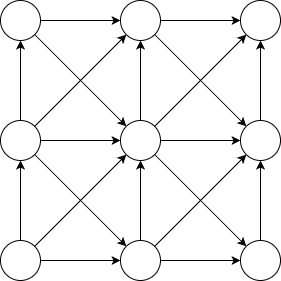
\includegraphics[width=0.3\textwidth]{../../res/membraneNeighbor.drawio}
    \caption{Illustration of neighbor relations in the membrane.}
    \label{fig:mem}
\end{figure}

\section{Parallelization}
\label{sec:para}

        The parallelization of our program primarily focused on parallelizing the force calulcation of the particles, as this posed the biggest computational effort in our program.
    \subsection{Implementing Thread-Safety}
In order to parallelize the iteration over all cells, every function in the iteration modifying shared data needed to be turned thread-safe. This especially included the \texttt{getNeighbours}-function of the \texttt{CellGrid} and the functions modifying a \texttt{Particle}.

\texttt{getNeighbourCells}:
\begin{itemize}
    \item{Initially, the \texttt{getNeighbourCells} proposed in the past assignments were meant to work under parallelization by simply adding locks to their respective function calls, but this was not true and modifications needed to be done.}
    \item{Whilst, a modification was found to be working for a static scheduleof the OMP-library, it surfaced that the concept of the function inheritly does not allow for parallelization.}
    \item{This is why we introduced \texttt{determineNeighboursStencile} in \texttt{CellGrid}, which pre-calculates the distinct neighbours of a \texttt{Cell} and stores it into \texttt{Cell.stencileNeighbours}. This follows the concept introduced in \texttt{Membrane}, calculating forces with half of the neighbours which are not symmetric to the center cell. }
\end{itemize}

\texttt{Particle}:
\begin{itemize}
    \item{In order to allow thread-safe modification of \texttt{Particle}, all functions were equipped with a lock, ensuring there were no race conditions.}
\end{itemize}

\subsection{Parallelization Strategy}
To compare different strategies, two parallelization strategies were implemented (static, task-based).
These can be chosen using the \texttt{-P} option via command line.
\bigskip

\textbf{Static parallelization}:
\begin{itemize}
    \item{We used the static schedule of \texttt{omp parallel for} to distribute cells amongst threads (see \texttt{force\_mixed\_LJ\_gravity\_lc}).}
    \item{This has great compatibility with the pre-calculated neighbours, as this tends towards a steady work load per cell rather than a dynamic behaviour, minimizing the wait time for the slowest thread. Still, if the cells themselves had big differences in the number of particles containing them, this could lead to a less optimal runtime.}
    \item{This strategy yields a runtime of around 45 seconds with 8 threads for the small 2D rayleigh experiment (commit: \texttt{923142a34003dec94c6dda462f4ef52704cd0983})}
\end{itemize}

\textbf{Task-based parallelization}:
\begin{itemize}
    \item{We used the task-based parallelization of \texttt{omp task} to distribute cells as a task amongst threads (see \texttt{force\_mixed\_LJ\_gravity\_lc\_task}).}
    \item{In this strategy, one thread iterates over the cells and creates tasks, which get dynamically assigned to threads. The dynamic nature of the task assignment might benefit if there was a great inbalance in the number of particles (workload) amongst the cells, so one might want to use this strategy in such scenarios. This strategy also has more additional overhead than the static parallalization, leading to a longer runtime if there is little difference in workload between the cells.}
    \item{This strategy yields a runtime of around 57 seconds with 8 threads for the small 2D rayleigh experiment (commit: \texttt{923142a34003dec94c6dda462f4ef52704cd0983})}
\end{itemize}

\subsection{Additional Parallelization}
It is not irrelevant to mention other parts of the program have been parallelized as well:
\begin{itemize}
    \item{The calculation of the location, the velocity of particles and the calculation used for the Thermostats have been parallelized. The iteration over the particles is distributed amongst threads using \texttt{omp parallel for}. Initially, a custom iterator (\texttt{ActiveIterator} in \texttt{ParticleContainer.h}) was implemented which only iterates over active (not deleted) particles and compatible for parallelization, but it was found that this was less performant than just iterating over the plain vector of particles and checking whether the particle is active or not. Though, the \texttt{ActiveIterator} might be superior in a scenario where a lot of particles get deleted, causing a bigger difference in workload between the threads.}
    \item{Though not relevant for the contest, we saw great interest in parallelizing the output of the simulation, as it was a significant part of the actual runtime. We succeeded in doing so by pre-allocating the buffer where particle information would be written and again distributing the particles to be written among threads using \texttt{omp parallel for} (see \texttt{VTKWriter.cpp}). Though, this faces the question at which index of the buffer a particle needs to be inserted, as we skip the inactive particles. Conveniently, each particle has an unique ID which is equivalent to the index it was put into the vector of the \texttt{ParticleContainer}. Subtracting the amount of inactive particles "before" the respective particle would result in our interesed "true" index of the particle. But how do we efficiently determine the number of inactive particles "before" one particle? Iterating through the vector and counting those would be a disaster for our runtime. To circumvent this, we take use of \texttt{std::map} and its tree structure over its keys. When "deleting" a particle, we insert its index (its ID) into this map (see \texttt{ParticleContainer:40}). This way we can now determine the number of deleted particles before a certain index by "following" the tree where it would insert us (see \texttt{ParticleContainer:47}), yielding a runtime of $n \cdot \log m$. With this, we can now parallelize the output of particles!}
\end{itemize}

\subsection{Parallelization Performance}
To verify the effectiveness of the parallelization, we ran the first 1000 iterations of the 3D rayleight experiment (\texttt{src/MolSim} \texttt{../input/reyleigh\_3D\_short.xml} \texttt{-x -s 4 -p}) on cm2\_tiny and cm2 clusters, using \texttt{scripts/}\texttt{batch-scripts/} \texttt{parallelComp.py}.
As seen below, initially we can observe an almost linear speedup as the number of threads increases, which then stagnates past 16 threads.
The concateneted output of the batch jobs (the runtimes) can be seen in \texttt{all.out} in our submission.

\bigskip

\centerline{
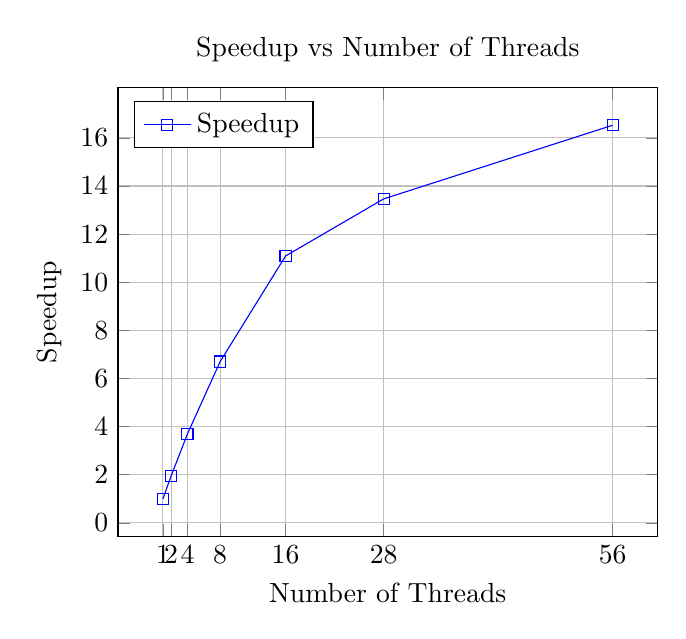
\begin{tikzpicture}
\begin{axis}[
    title={Speedup vs Number of Threads},
    xlabel={Number of Threads},
    ylabel={Speedup},
    grid=both,
    xtick={1, 2, 4, 8, 16, 28, 56},
    ytick={0, 2, 4, 6, 8, 10, 12, 14, 16},
    legend pos=north west
]
\addplot[
    color=blue,
    mark=square,
    ]
    coordinates {
    (1, 1)
    (2, 3272 / 1680)
    (4, 3272 / 885)
    (8, 3272 / 488)
    (16, 3272 / 295)
    (28, 3272 / 243)
    (56, 3272 / 198)
    };
\addlegendentry{Speedup}
\end{axis}
\end{tikzpicture}
}

\bigskip
We also analysed the runtime distribution using \texttt{gprof}.
The distribution when running \texttt{src/MolSim} \texttt{../input/small\_rayleigh\_taylor.xml} \texttt{-x -s 4 -P static} at commit \texttt{923142a34003dec94c6dda462f4ef52704cd0983} with 8 cores can be seen in Figure \ref{fig:runtime}.
Nodes and edges with less than 0.5\% runtime have been left out for a simpler overview.
We can observe that the most time is spent at computing the forces, of which a third is the raw calculation of Lennard Jones forces.
We interpret this positively, as we spend most our time of the program for the heart of the simulation, the force calculation, which is also the tackle point of our parallelization.
Furthermore, we can see that we significantly reduced the runtime of the output of particles to essentially the I/O operation of the file (\texttt{VTKFile} is 6.36\% of 6.41\% of \texttt{writeFile}).
Additionally, location, velocity calculation and the thermostat calculations are below 0.5\% of the total runtime.
Another significant of the runtime is the \texttt{\_init} function, which is called when a shared library is loaded.
As we do not use any libraries except \texttt{spdlog}, \texttt{xerces-c} and \texttt{openmp}, we interpret this as an indicator that our overall runtime of our program is quite low, but we might need to investigate this further :)

\begin{figure}[H]
    \centering
    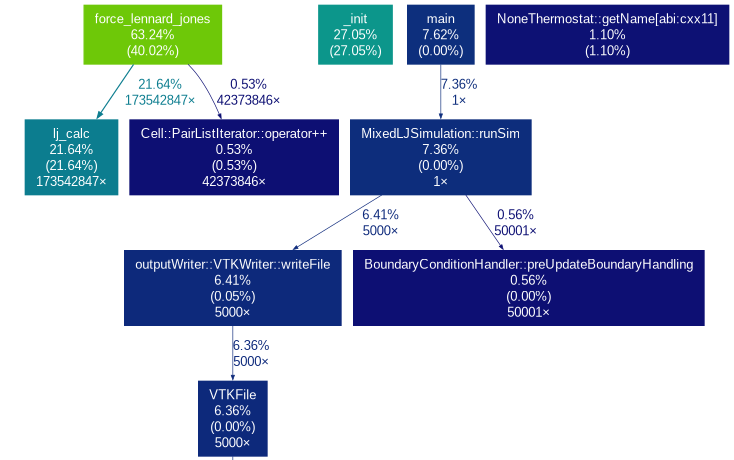
\includegraphics[width=1\textwidth]{../../res/optimized.png}
    \caption{Visualization of runtime distributions.}
    \label{fig:runtime}
\end{figure}

\section{Rayleigh-Taylor instability in 3D}
This experiment is specified in \texttt{reyleigh\_3D.xml}.
We ran the simulation using 18 cores, which took a bit more than 20 hours, with an output frequency of every 10 iterations.
The final result of our simulation can be found \href{https://www.youtube.com/watch?v=DXrORoIFdDM}{here}.
We can observe how the upper fluid finds multiple entrypoints, forcing its way down.
Finally, the fluids switch places and start to stabilize.


For a thrilling acoustic experience, we also created a heavy metal version of the \href{https://youtu.be/U99R1vSeBxQ}{experiment}, emphasizing the blood, sweat and tears that have flown for this project.

\section{Competition}
We are thrilled to find out how good our program is compared to the other teams!
Unfortunately, compiling in g++/11 on the cluster did not work, as it does not allow the usage of enhanced for loops.
To overcome this, we would need to change the code on a lot of spots to less readable one, which we decided against. 
We still hope that we can convince you with our program and our hard dedication!!
\textbf{Note}: The output says 999 iterations, but we also count the zeroth iteration. 
You can also find the output files of the batch jobs in this submission.

\bigskip
This is our best runtime for the 3D experiment with the following specifications:

\begin{itemize}
    \item 56 threads 
    \item cluster: cm2
    \item partition: cm2\_std
    \item time: 198s
    \item compiler: icpc
    \item xml: \texttt{reyleigh\_3D\_short.xml}
\end{itemize}

Batch job output:
\begin{lstlisting}
[2024-07-17 14:05:46.499] [info] Simulation ran for 198 seconds (999 iterations)
[2024-07-17 14:05:46.501] [info] Average time per iteration: 198 ms
[2024-07-17 14:05:46.501] [info] MUP/S = 505050 (MUP = force+vel+pos calc i.e. one update per particle per iteration)
[2024-07-17 14:05:46.501] [info] Output written. Terminating...
\end{lstlisting}
You can recreate this using the latest commit on the \texttt{assignment5} branch and then submitting the batch job via \texttt{parallel\_56.sh} found in this submission.


\bigskip
This is our best runtime for the 2D experiment with the following specifications:

\begin{itemize}
    \item 16 threads 
    \item cluster: cm2
    \item partition: cm2\_std
    \item time: 2s 
    \item compiler: icpc
    \item xml: \texttt{big\_rayleigh\_taylor\_short.xml}
\end{itemize}

Batch job output:
\begin{lstlisting}
[2024-07-18 15:01:49.698] [info] Simulation ran for 2 seconds (999 iterations)
[2024-07-18 15:01:49.698] [info] Average time per iteration: 2 ms
[2024-07-18 15:01:49.698] [info] MUP/S = 5000000 (MUP = force+vel+pos calc i.e. one update per particle per iteration)
[2024-07-18 15:01:49.698] [info] Output written. Terminating...
\end{lstlisting}
You can recreate this using the latest commit on the \texttt{assignment5} branch and then submitting the batch job via \texttt{brl\_parallel\_16.sh} found in this submission.



\section{Nano-scale flow simulation}
\label{sec:nano}

The nano flow simulations did not require new physics and had most of the elements in place \textit{a priori}, which is why we decided to tackle option A.

\subsection{Experimental setups}
\label{sec:nano:exp}

    \begin{itemize}
        \item We performed a series of 5 simulations, investigating different experimental settings
        \item Generally, we would expect the fluid particles to accelerate in the y-direction due to gravity
        \item The wall particles are fixed and should by their attractive forces slow nearby particles
        \item[] \!\!\!\!\!\!\!\!\! $\Rightarrow$ We expect to see a concave graph along the velocity profiles and thus a more blue coloring in the center, while the particles closer to the walls should be more red. The density profile should also be higher towards the center as particles are dragged into the center by the higher velocities.
        \item \textbf{Some general notes:} The spikes in the density profile on the edges and the zero-velocities on the edges are due to the walls and the relatively fine grained grid (50 bins in x, 20 bins in z).
    \end{itemize}

    \begin{enumerate}
        \item Base simulation: We ran the simulation as specified on the worksheet with the following parameters and results:
        \begin{itemize}
            \item $g_{grav} = -0.8$
            \item $n_{thermostat} = 10$
            \item $\epsilon_{wall} = 2.0$, $\sigma_{wall} = 1.1$
            \item $\epsilon_{fluid} = 1.0$, $\sigma_{fluid} = 1.0$
            \item Unfortunately, the simulation was terminated before finishing on the cluster (at 67\%)
            \item Looking at the video of the simulation and corresponding profiles (see Section \ref{sec:nano:video}), one is not able to see any form of acceleration of the particles in the center
            \item Also visibly no acceleration along the y-axis can be made out
            \item The density profile also remains unchanged
        \end{itemize}
        \item We suspected the analyzer was not able to measure the fine changes in velocity, as the analyzer only wrote the mean $||V||_{l2}$ to the file. The y-velocity changes might have been more prominent. Thus we restarted the simulation with the following:
        \begin{itemize}
            \item $g_{grav} = -0.8$
            \item $n_{thermostat} = 10$
            \item $\epsilon_{wall} = 2.0$, $\sigma_{wall} = 1.1$
            \item $\epsilon_{fluid} = 1.0$, $\sigma_{fluid} = 1.0$
            \item \textbf{Only change:} Analyzer now writes the mean velocities only along the y-axis $\; \frac{1}{\text{\#Bin Particles}}\sum_{p}^{\text{Bin Particles}} p.vel.y$
            \item However, looking at the velocity profile in the y-direction does still not reveal the expected result.
            \item The mean velocity in y-direction seems to be evenly distributed in both positive and negative to yield zero in the end, i.e. no directed flow seems to take place
            \item We hypothesized this could be due to weak wall-fluid interactions and a weak gravity force, and/or the thermostat being applied to often to not allow for acceleration downward.
            \item Which then ends up in a random flow that has no directed downward movement
            \item \textbf{Please note:} The video says the max iteration to be 8214 instead of 10000. This is due to some vtk files being missing after copying them to the local machine. We are not certain, how this could have happened.
        \end{itemize}
        \item Building upon the last experiment we decided to increase $\epsilon$ and decrease $\sigma$ to force stronger wall-fluid interactions as well as increasing the thermostat frequency and gravity to allow for stronger acceleration.
        \begin{itemize}
            \item $g_{grav} = -9.81$
            \item $n_{thermostat} = 1000$
            \item $\epsilon_{wall} = 2.0$, $\sigma_{wall} = 1.1$
            \item $\epsilon_{fluid} = 5.0$, $\sigma_{fluid} = 0.8$
            \item The idea being that the wall would attract nearby particles more strongly while center particles would accelerate more strongly by the increased gravity
            \item Looking at the video one can see that the thermostat frequency was set way to high, leading to an inevitable explosions as the velocities continuously increase
        \end{itemize}
        \item Thus the next idea was decreasing the thermostat's frequency back to the default value provided on the worksheet to control the temperature. The results finally approached our expectations:
        \begin{itemize}
            \item $g_{grav} = -9.81$
            \item $n_{thermostat} = 10$
            \item $\epsilon_{wall} = 2.0$, $\sigma_{wall} = 1.1$
            \item $\epsilon_{fluid} = 5.0$, $\sigma_{fluid} = 0.8$
            \item Looking at the video one can observe a formation of the expected concave velocity graph (now back to l2 norm, video is mis-labeled)
            \item Also the density is slightly higher in the center compared to closer to the wall
            \item This can be explained by the particles essentially being packed as close together as possible from the beginning, not allowing for a lot of compression, thus only a tiny increase can be observed
            \item Also visually it can be nicely seen that the center particles are more blue than the edges confirming the profile
        \end{itemize}
        \item Unrelated to the other experiments, we wanted to see if we could observe turbulences. We placed a small 2 by 10 particle cluster at the edge of the flow while leaving the other parameters to their default values.
        \begin{itemize}
            \item $g_{grav} = -0.8$
            \item $n_{thermostat} = 10$
            \item $\epsilon_{wall} = 2.0$, $\sigma_{wall} = 1.1$
            \item $\epsilon_{fluid} = 1.0$, $\sigma_{fluid} = 1.0$
            \item Unfortunately, the small cluster did not impact the flow as that we could observe it.
            \item Also, as the default setup does not seem to generate a directed flow no turbulences could be expected.
            \item Looking at the velocity profile does not show any decrease in the center where the cluster is underling the hypothesis no directed flow is occurring in the base simulation.
            \item As the simulations took a long time to run and we had to finish the sheet, we decided against running follow-up experiments.
            \item It would however have been interesting to run the same simulation with the parameters of the stronger wall simulation and look for any turbulences.
        \end{itemize}
        
    \end{enumerate}

\subsection{Videos}
\label{sec:nano:video}

    \begin{itemize}
        \item Here a list of all videos for the simulation.
        \item The coloring of the simulation is by the velocities along the y-axis, where smaller numbers suggest downward movement (darker blue color), while larger numbers suggest upward movement (red color).
        \item The simulations below are the ones specified above in Section \ref{sec:nano:exp}
        \begin{enumerate}
            \item Standard simulation run (until t=30): \href{https://youtu.be/-eWISjhgIgA}{here}
            \item Standard simulation run. Full run, only y-direction profile: \href{https://www.youtube.com/watch?v=0xr62UzcphU}{here}
            \item Stronger wall-fluid interactions, stronger gravity, less frequent thermostat: \href{https://www.youtube.com/watch?v=yxNYmXJg5r0}{here}
            \item Stronger wall-fluid interactions, stronger gravity: \href{https://www.youtube.com/watch?v=I4h6tjnJVuI}{here}
            \item Addition of small cluster of particles: \href{https://www.youtube.com/watch?v=G34H3SCnpW0}{here}
        \end{enumerate}
    \end{itemize}

\subsection{Implementation of the flow simulation}
\label{sec:nano:impl}

    \subsubsection{Immobilization}
    \label{sec:nano:impl:immob}
        \begin{itemize}
            \item To fix particles and make them immovable, we added a new input specification where particle types could be marked immobile.
            \item For that we had to introduce a new boolean attribute to particles to mark them as stationary.
            \item Within the velocity and positional calculations, we disregard any particles that are immobilized.
            \item Adjustments were made to the generation, boundary, and calculation files to accommodate stationary particles.
            \item The feature of immobile particles is backwards compatible so that even the base simulation has the option to have immobile particles.
        \end{itemize}

    \subsection{Thermostat}
    \label{sec:nano:impl:thermo}
        \begin{itemize}
            \item For the nano flow simulation a new thermostat class was implemented - \texttt{thermostat/IndividualThermostat}
            \item This thermostat will ignore fixed particles and perform temperature updates without changing the mean velocity of the particles.
            \item The selection of the thermostat is now decided via a factory function. The thermostat can be turned off by selecting the \texttt{NoneThermostat} or setting the frequency of thermal updates to 0.
            \item This approach allowed us to run the simulation without creating a new simulation class and by simply specifying simulation parameters.
        \end{itemize}


\subsection{Analytics}
\label{sec:nano:ana}

    \begin{itemize}
        \item We added a class \texttt{analytics/Analyzer} that can write density and velocity profiles to a .csv file for later analysis.
        \item The specification of analysis frequency and output file name can be done using the xml attributes.
        \item Also, it is possible to specify the number of bins to look at. This is even possible in multiple dimensions, allowing for more fine-grained analytics.
        \item As the .csv is only in 1D we needed to flatten the data using the following formula:
        \[
        \text{1D Index} = \text{x-Index} + \text{y-Index} \cdot \text{\#x-Bins} + \text{z-Index} \cdot \text{\#x-Bins} \cdot \text{\#y-Bins}
        \]
        \item The resulting profiles can then be plotted to a 2D heat map and 2D graph via a python script in \texttt{scripts/plots}.
        \item In our simulations we decided to have bins in 2 dimensions. The resulting heat map can be interpreted as the velocity / density profile of slices on top of the x-z-plane. The graph is simply the collapsed version onto the x-axis (see Figure \ref{fig:plot_xmpl}).
        \item In the videos of the nano flow simulations in Section \ref{sec:nano:video} the plotted diagrams for density and velocity can be seen next to the running simulation.
        \item Regarding feedback from previous assignments and continuously increasing run-times, we added a progress logger to let the user know about the estimated time the simulation will still take to complete.
        \item This is also a nice quality of life feature as it is a simple sign that the simulation is progressing
    \end{itemize}

    \begin{figure}[H]
        \centering
        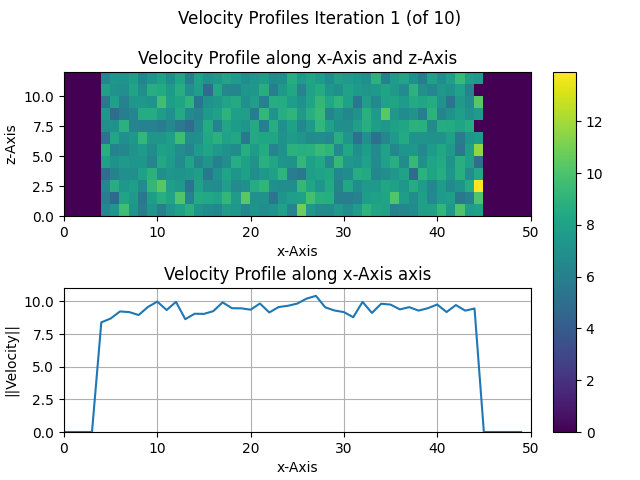
\includegraphics[width=1\textwidth]{../../res/Profile_example.png}
        \caption{Example of our profiling plots. The heat map is a visualization of velocities along the y-axis on top of the x-z plane. The graph is the collapsed versions onto the x-axis. }
        \label{fig:plot_xmpl}
    \end{figure}

    \begin{itemize}
        \item Even though the assignment did not call for it, we implemented a python script to get the same metrics from the .vtk files allowing us to generate statistics even after the simulation has run (scripts/plots/vtk2velProfile.py).
        \item This might be a good point to expand the analytical capabilities, as the simulation must nor be re-run to obtain the analytics.
    \end{itemize}

\end{document}
